データとは、計算機が扱うことのできる情報の形式と考えることができる。
この意味では、データを理解するためには計算機の構造をある程度理解する必要があることを述べておく。
このことは「データ処理とは」の章でもう少し詳しく解説するが、本書では端的には「電子計算機が扱うことのできるバイト列またはビット列」を指す。
\begin{breakbox}
$\Rightarrow$ 電子計算機以外にどのようなタイプの計算機があるか調べてみよう。
\end{breakbox}

\subsection{データ型}
一般的にデータ型とはデジタル電子計算機が扱うデータフォーマットのことと考えてよい。データ型には幾つかの抽象化レベルがあるが、最下層としては単なるビット列をどのように解釈するかである。すなわち、例えば以下のようなものである。
\begin{itemize}
\item 整数型
\item 小数(浮動小数点数)型
\item 文字型
\end{itemize}
\begin{breakbox}
$\Rightarrow$ 上記以外にどのようなデータ型があるか調べてみよう。
\end{breakbox}

\subsection{文字と文字列}
ここで、文字と数字、文字列について述べておこう。
文字は文字コードによって解釈されるが、文字コードはさらにエンコードされている。
UTF8とは、ユニコードをエンコードする一つの方法である。数字とは、数を表すための文字であり、数値とは異なる。
数値とは前述したように、整数や小数という概念そのもの、あるいは計算機上で数値として取り扱うビット列のことである。
文字列とは文字コードまたは文字エンコードの並らびである。
数値は、数字列によって表現されることが一般的である。
直接バイナリ記述される場合もある。
\begin{breakbox}
$\Rightarrow$ このことをCの\shortstack[l]{sscanf()}などで確認しよう。

$\Rightarrow$ リトルエンディアンとは何か調べてみよう。
\end{breakbox}

\subsection{集合、リスト、ツリー、グラフ}
\begin{figure}
\begin{center}

\begin{tabular}{c}
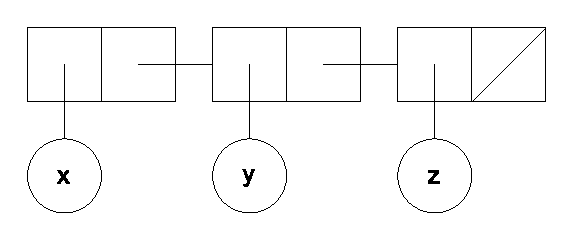
\includegraphics[width=8cm]{list_xyz.eps} \\
�ꥹ��(x,y,z)��ɽ�����ꥹ�ȹ�¤ \\
\\
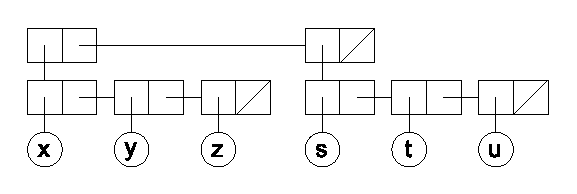
\includegraphics[width=8cm]{list_xyz-stu.eps} \\
�ꥹ��((x,y,z),(s,t,u))��ɽ�����ꥹ�ȹ�¤(����) \\
\end{tabular}

\caption{\label{zu-cell} [�ꥹ�ȹ�¤]}
\end{center}
\end{figure}

\begin{figure}[h]
\begin{center}

\begin{tabular}{c}

\includegraphics[width=8cm]{zu-gr.eps} \\
����դΥ���ե�����ɽ�� \\
\\
%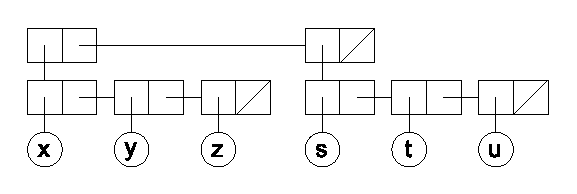
\includegraphics[width=8cm]{list_xyz-stu.eps} \\
\begin{math}
\left(
\begin{array}{cccc}
 0 & 1 & 1 & 1 \\
 1 & 0 & 0 & 0 \\
 1 & 0 & 0 & 1 \\
 1 & 0 & 1 & 0 \\
\end{array}
\right)
\end{math} \\
����դ����ܹ���ɽ�� \\
\end{tabular}

\caption{\label{zu-graph} [����չ�¤]}
\end{center}
\end{figure}

一般的にデータを取り扱う際にはデータ単体(datum)の単位では扱わず、データ集合として扱う。
ここで言う集合は一般的な集合ではなく、一種の配列、つまり、要素の並び順や重複に意味があるものである。
リストとは、要素を並べただけのものから、より高位の階層構造などを表すために用いられる表現である。
最も代表的な構造はCons Cellであり、文字列による表現ではカッコ()によって階層を表し、内部実装としてはポインタによるセルの連結である[Figure:\ref{zu-cell}]。
近年よく用いられるJSON形式は一種のリスト表現である。
ツリーは基本的にはリストと同じで、分岐のあるリストを特にツリーと称する。
この場合も内部実装はCons Cellで現すことができる。
グラフはより高位の構造であり、抽象レベルの表現、内部実装ともに複雑になるが、これらを表現する幾つかの方法がある。
その一つは隣接行列を利用することである[Figure:\ref{zu-graph}]。

グラフよりもさらに高次な構造も当然ある。
グラフの均質化やラベル付与は、より複雑なネットワーク構造を表す\cite{FujiwaraYuzuru}。
いずれの構造を表わすにおいても、前述のリスト構造がデータ構造における基本と考えてよい。

\begin{breakbox}
$\Rightarrow$ 配列とポインタ参照 \\
プログラミング言語ではよくポインタが使用されるが、Javaのような近代的な言語はその効果が隠蔽されており、解り難い。
C言語においてすらポインタ参照と配列参照はカッコ[]と引数で表現され、違いがない。
しかし、次のようなコードでその違いを確認できる。
\begin{center}
==========Start of code==========
\end{center}
\scriptsize
\begin{verbatim}
/* データサイズをprintする */
#include <stdio.h>
#include <stdlib.h>

int main(){
        printf("int             \t:%ld:\tbyte\n",sizeof(int));
          int a[2][2];
        printf("int 2D:2x2      \t:%ld:\tbyte\n",sizeof(a));
        printf("pointer int*    \t:%ld:\tbyte\n",sizeof(int*));
        return(0);
}
\end{verbatim}
\normalsize
\begin{center}
==========End of code==========
\end{center}
出力は以下となる。
\begin{center}
==========Start of print==========
\end{center}
\scriptsize
\begin{verbatim}
int             	:4:	byte
int 2D:2x2      	:16:	byte
pointer int*    	:8:	byte
\end{verbatim}
\normalsize
\begin{center}
==========End of print==========
\end{center}
\end{breakbox}

\subsection{メタデータ}
蛇足ながら、メタデータについて述べておく。
メタデータはデータを説明するためのデータであり、何がメタデータであるかは、個々のシステム、個人により定義されるが、明確に定義されない場合もある。
データが形式的になるほど、何がメタデータで何がデータなのかという区別は不要になっる。
すなわち、データ構造が完全に形式的に定義され、その解釈も一意に決まる場面では、メタデータという概念は不要である。

